% !TEX spellcheck = en_US

The steady states are influenced by the design of the controller and turbine in the simulation. These states are useful for initializing the simulation, as they provide essential information for analyzing the turbine's power behavior and the controller settings. Additionally, these steady states play a crucial role in the overall wind turbine design and can be utilized to initialize further simulations.

The general procedure we followed to find the steady-state parameters is as follows: 
\begin{itemize}
	\item First, find the rated wind speed. 
	\item Then, calculate the steady states below the rated wind speed separately for regions 1, 1.5, 2, and 2.5. 
	\item Finally, calculate the steady states above the rated wind speed.
\end{itemize}

Find the $v_{rated}$, $v_{1to1.5}$, $v_{1.5to2}$ and $v_{2to2.5}$ using the minimization problem method, as show in Equation \ref{equation:Minimization problem}. Also, use the minimization problem method to find the above-rated wind speed, as shown in the equation  \ref{equation:Minimization problem above rated wind}.

\begin{equation}
	\min_{v_0} \left( M_a(v_0, \Omega, \theta) - M_G \right)^2
	\label{equation:Minimization problem}
\end{equation}

\begin{equation}
	\min_{\theta} \left( M_a(v_0, \Omega, \theta) - M_G \right)^2
	\label{equation:Minimization problem above rated wind}
\end{equation}

In 5MW Optimus-Shakti simulation model are performed for complete wind bins ranging from 0 to 30 m/s. To determine if the simulation has stabilized, the standard deviation of the tower top displacement is calculated. The values for wind speed, pitch angle, rotor speed, tip speed ratio, generator torque, and the standard deviation of the nacelle acceleration are determined. Additionally, the results are visually assessed through plots. The values found through simulation are $v_{rated} = 9.3531$, $v_{1to1.5} = 6.0652$, $v_{1.5to2} = 6.0652$ and $v_{2to2.5} = 8.6631$. Figure \ref{fig:power cureve} demonstrates the model's static behavior by plotting power against wind speed.

\begin{figure}[htbp]
	\centering
	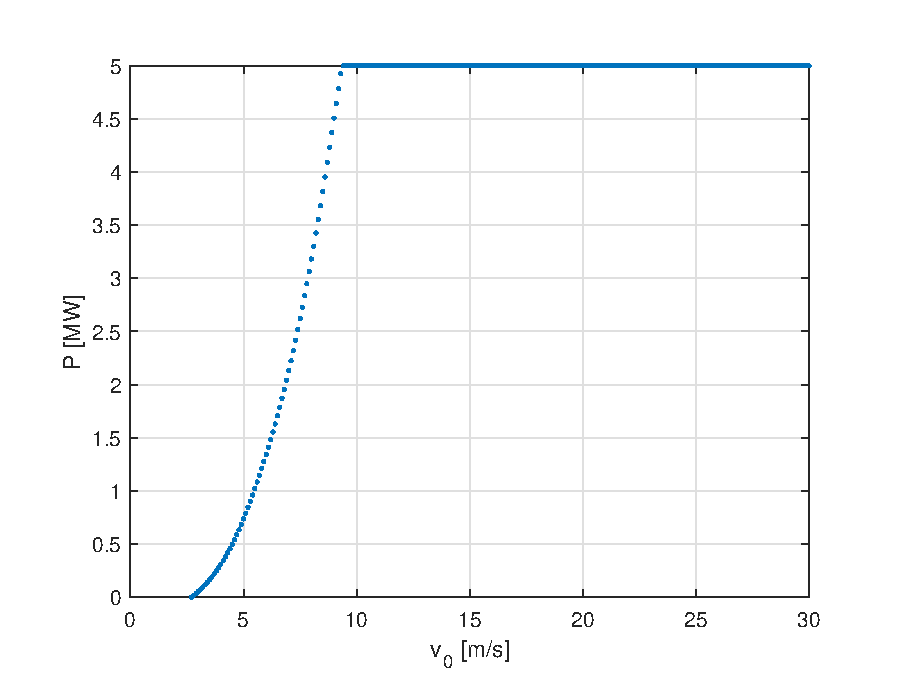
\includegraphics[width=0.7\textwidth]{Figures/P_Vs_v.eps}
	\caption{Power curve calculated with steady state calculations}
	\label{fig:power cureve} 
\end{figure}
